% !TEX root = main.tex

\section{Linear Hyperbolic Partial Differential Equations}

%%%%%%%%%%%%%%%%%%%%%%%%%%%%%%%%%%%%%%%%%%%%%%%%%%%%%%%%%%%%%%%%%%
\subsection{The Radiative Transfer Problem}
\begin{align*}
	F_{,t} + \vec{\Omega} \cdot \vec{\nabla}F + \sigma_t F = \frac{\sigma_s}{4\pi}\int_{\mathbb{S}^2}F\, d\vec{\Omega}
\end{align*}
The radiative transfer problem is one of great interest in computational mathematics.
It serves as a kinetic model for subatomic particles propagating through a homogeneous medium, where $F(t, \vec{x}, \vec{\Omega}): \mathbb{R}^+ \times \mathbb{R}^3 \times \mathbb{S}^2 \to \mathbb{R}$ is a distribution for particles at position $\vec{x}$ with velocity $\vec{\Omega}$. The equation itself is linear, but the solution function is expressed in $5 + 1$ dimensions.
As a result, it is exceptionally difficult to discretize and solve immediately, and a significant amount of effort is put in to reduce the number of dimensions present.

The first such effort comes from the spherical harmonics expansion, a series expression that isolates the dependencies of the $\vec{\Omega} = [\mu \, \phi]^T$ variables. 
Because the terms $Y_\ell^m$ are already known by construction, we are left to calculate the $F_\ell^m$ terms.
Moreover, we only consider the 2D case.
\begin{align*}
	F(t, \vec{x}, \vec{\Omega}) \approx \sum_{\ell = 0}^N \sum_{m=-\ell}^\ell F_\ell^m(t, \vec{x})Y_\ell^m(\mu, \phi)
\end{align*}
Taking the first $N$ terms of this series, we can substitute it into the original radiative transfer equation.
Algebraic manipulation\cite{BrunnerHolloway:1} reveals $\frac{1}{2}(N+1)(N+2)$ equations combined into a system of linear partial differential equations of the following form:
\begin{align*}
	\vec{F}_{,t} + \mat{A}\,\vec{F}_{,x} + \mat{B}\,\vec{F}_{,y} & = \mat{C}\,\vec{F}
\end{align*}
Note that we have reduced our $5+1$ dimensional equation to one in $2+1$ dimensions.
We then apply our Radon transform to the PDE to remove an additional spatial derivative, as we will see.
%%%%%%%%%%%%%%%%%%%%%%%%%%%%%%%%%%%%%%%%%%%%%%%%%%%%%%%%%%%%%%%%%%
\subsection{Radon Transforms of Partial Derivatives}

We consider the following system of $M$ first-order, linear hyperbolic PDEs:
\begin{align*}
	\vec{q}_{,t} + \mat{A}\,\vec{q}_{,x} + \mat{B}\,\vec{q}_{,y} & = \mat{C}\,\vec{q} \\
	\vec{q} \left( t = t_0, x, y \right) & = \vec{q_0} \left( x, y \right)
\end{align*}
where 
\begin{itemize}
    \item $\vec{q}(t, x, y): \mathbb{R}^{+} \times \mathbb{R}^{2} \rightarrow \mathbb{R}^{M}$ is a vector valued function of time and space
    \item $\mat{A}, \mat{B}, \mat{C} \in \mathbb{R}^{M \times M}$ are constant matrices
    \item $\vec{q_{0}}(x, y) \in \mathbb{R}^{M}$ is a vector of initial conditions
\end{itemize}
We can apply the Radon transform to the above PDE and and use the properties of the transform to simplify spatial partial derivatives.
\begin{align}
	& \mathcal{R}{\left( \vec{q}_{,t} + \mat{A}\, \vec{q}_{,x} + \mat{B} \, \vec{q}_{,y} = \mat{C} \, \vec{q} \right)} \\
	\implies & \mathcal{R}{\left( \vec{q}_{,t} \right)} + \mathcal{R}{\left( \mat{A} \, \vec{q}_{, x} \right)} + \mathcal{R}{\left( \mat{B} \, \vec{q}_{, y} \right)} = \mat{C} \, \mathcal{R}{\left( \vec{q} \right)} \\
	\implies & \mathcal{R}{\left( \vec{q}_{,t} \right)} + \mat{A} \,\mathcal{R}{\left(  \vec{q}_{, x} \right)} + \mat{B} \,\mathcal{R}{\left(  \vec{q}_{, y} \right)} = \mat{C} \, \mathcal{R}{\left( \vec{q} \right)} \\
	\implies & \widehat{\vec{q}}_{, t} + \cos \left( \omega \right) \, \mat{A} \, \widehat{\vec{q}}_{, s} + \sin \left( \omega \right) \, \mat{B} \, \widehat{\vec{q}}_{, s} = \mat{C} \, \widehat{\vec{q}} \\
	\implies & \vec{\widehat{q}}_{,t} + \left( \cos \left( \omega \right) \, \mat{A} + \sin \left( \omega \right) \, \mat{B} \, \right) \vec{\widehat{q}}_{,s} = \mat{C}\,\vec{\widehat{q}}
\end{align}
In $(2)$ and $(3)$, we use the linearity of the Radon transform to apply it separately to each term of the PDE.
In $(4)$ and $(5)$, we use the intertwining property of the Radon transform (as discussed earlier) to simplify spatial partial derivatives.
\par
\textbf{Note:} We have only taken the Radon transform of the PDE at one angle $\omega$.
\par
After applying the Radon transform to the PDE and its corresponding initial condition, we obtain the following:
\begin{align}
    \vec{\widehat{q}}_{,t} + \left( \cos \left( \omega \right) \, \mat{A} + \sin \left( \omega \right) \, \mat{B} \, \right) \vec{\widehat{q}}_{,s} & = \mat{C}\,\vec{\widehat{q}} \\
    \widehat{\vec{q}} \left( t = 0, s, \omega \right) & = \widehat{\vec{q_0}} \left( s, \omega \right)
\end{align}
Take $\widetilde{\mat{A}} \left( \omega \right) :=  \cos \left( \omega \right) \, \mat{A} + \sin (\omega) \, \mat{B}\,$ and substitute $\widetilde{\mat{A}} \left( \omega \right)$ into $\left( 6 \right)$ to obtain the following:
\begin{align}
	\vec{\widehat{q}}_{,t} + \widetilde{\mat{A}} \left( \omega \right) \vec{\widehat{q}}_{,s} & = \mat{C}\,\vec{\widehat{q}} \\
	\widehat{\vec{q}} \left( t = 0, s, \omega \right) & = \widehat{\vec{q_0}} \left( s, \omega \right)
\end{align}

\subsection{Discretization of the PDE}

\subsubsection{Hyperbolicity}

Recall that we are working with a system of first-order, linear hyperbolic PDEs.
In this context, the system is \textbf{hyperbolic} if $\widetilde{\mat{A}} \left( \omega \right)$ (which was defined earlier) is diagonalizable with only real eigenvalues for all $\omega \in \mathbb{R}$.
\par 
This means $\widetilde{\mat{A}} \left( \omega \right)$ admits the following factorization:
\begin{align}
    \widetilde{\mat{A}} \left( \omega \right) = \mat{P} \, \mat{\Lambda} \, \mat{P}^{-1}
\end{align}
where
\begin{itemize}
    \item $\mat{P}$ is a matrix whose columns are the eigenvectors of $\widetilde{\mat{A}} \left( \omega \right)$
    \item $\Lambda$ is a diagonal matrix whose entries are the eigenvalues of $\widetilde{\mat{A}} \left( \omega \right)$
\end{itemize}

%%%%%%%%%%%%%%%%%%%%%%%%%%%%%%%%%%%%%%%%%%%%%%%%%%%%%%%%%%%%%%%%%%
\subsubsection{Using the Hyperbolicity of the PDE}

Recall that we have transformed our system of $M$ first-order, linear hyperbolic PDEs into the following family of systems of first-order, linear hyperbolic PDEs
\begin{align}
    \vec{\widehat{q}}_{,t} + \widetilde{\mat{A}} \left( \omega \right) \vec{\widehat{q}}_{,s} & = \mat{C}\,\vec{\widehat{q}} \\
	\widehat{\vec{q}} \left( t = 0, s, \omega \right) & = \widehat{\vec{q_0}} \left( s, \omega \right)
\end{align}
for each angle $\omega$.
\par 
We can use the eigendecomposition of $\widetilde{\mat{A}} \left( \omega \right)$ to rewrite $\left( 11 \right)$:
\begin{align}
    \widehat{\vec{q}}_{,t} & + \widetilde{\mat{A}}(\omega) \, \widehat{\vec{q}}_{,s} = \mat{C} \, \widehat{\vec{q}} \\
    \Rightarrow \,  \widehat{\vec{q}}_{,t} & + \mat{P} \, \mat{\Lambda} \, \mat{P}^{-1} \, \widehat{\vec{q}}_{,s} = \mat{C} \, \widehat{\vec{q}} \\
    \Rightarrow  \mat{P}^{-1} \,  \widehat{\vec{q}}_{,t} & + \mat{\Lambda} \, \mat{P}^{-1} \, \widehat{\vec{q}}_{,s} = \mat{P}^{-1} \, \mat{C} \, \widehat{\vec{q}} \\
    \Rightarrow  \frac{\partial}{\partial t}  \left(\, \mat{P}^{-1} \,   \widehat{\vec{q}} \, \right) & + \mat{\Lambda} \, \frac{\partial}{\partial s} \left(\, \mat{P}^{-1} \, \widehat{\vec{q}} \,\right) = \mat{P}^{-1} \, \mat{C} \, \widehat{\vec{q}}
\end{align}
We can take $\vec{w} := \mat{P}^{-1} \, \widehat{\vec{q}}$ to be the vector of \textbf{characteristic variables} and rewrite $\left( 16 \right)$:
\begin{align*}
    \vec{w}_{, t} + \mat{\Lambda} \, \vec{w}_{, s} = \mat{P}^{-1} \, \mat{C} \, \mat{P} \, \vec{w}
\end{align*}
We can now introduce $\mat{F} := \mat{P}^{-1} \, \mat{C} \, \mat{P}$ and obtain the following family of systems of partially decoupled first-order, linear PDEs
\begin{align*}
    \vec{w}_{, t} + \mat{\Lambda} \, \vec{w}_{, s} & = \mat{F} \, \vec{w} \\
    \vec{w}(t = 0, s, \omega) & = \vec{w_{0}}(s, \omega) 
\end{align*}
for each angle $\omega$.
\par
\textbf{Note:} The above system is generally only partially decoupled. 
The system is fully decoupled if $\mat{C} \equiv \mat{0}$.

\subsubsection{Spatial Discretization of the PDE}

Recall for a fixed angle $\omega$, we are working with the following system of first-order, linear hyperbolic PDEs:
\begin{align*}
    \vec{w}_{, t} + \mat{\Lambda} \, \vec{w}_{, s} & = \mat{F} \, \vec{w} \\
    \vec{w}(t = 0, s, \omega) & = \vec{w_{0}}(s, \omega) 
\end{align*}
The $p^{th}$ equation in the system is given explicitly as follows:
% \begin{align*}
%     w_{p, t} + \lambda_{p} w_{p, s} = \sum_{q=1}^{M} F_{pq} w_{q} \quad \rightarrow \quad 
%     \vec{W_{p}}_{, t} + \lambda_{p} \vec{W_{p}}_{, s} = \sum_{q=1}^{M} F_{pq} \, \vec{W_{q}}
% \end{align*}
\begin{align*}
    w_{p, t} + \lambda_{p} w_{p, s} = \sum_{q=1}^{M} F_{pq} w_{q}
\end{align*}
We need to discretize the above system to computationally work with it.
\par 
We do this by discretizing the $p^{th}$ equation in space, and we naturally approximate $w_{p}$ at $N_{s}$ many Chebyshev points of the second kind along the line determined by the angle $\omega$:
\begin{align}
    w_{p} \rightarrow \vec{W_{p}} \in \mathbb{R}^{N_{s}}
\end{align}
Thus,
\begin{align}
     w_{p, t} + \lambda_{p} w_{p, s} = \sum_{q=1}^{M} F_{pq} w_{q} \quad \rightarrow \quad 
    \vec{W_{p}}_{, t} + \lambda_{p} \, \vec{W_{p}}_{, s} = \sum_{q=1}^{M} F_{pq} \, \vec{W_{q}}
\end{align}
We now need to discretize the spatial derivative operator, and we naturally use the Chebyshev spectral differentiation matrix $\mat{D} \in \mathbb{R}^{N_{s} \times N_{s}}$
% \begin{figure}[H]
% 	\centering
% 	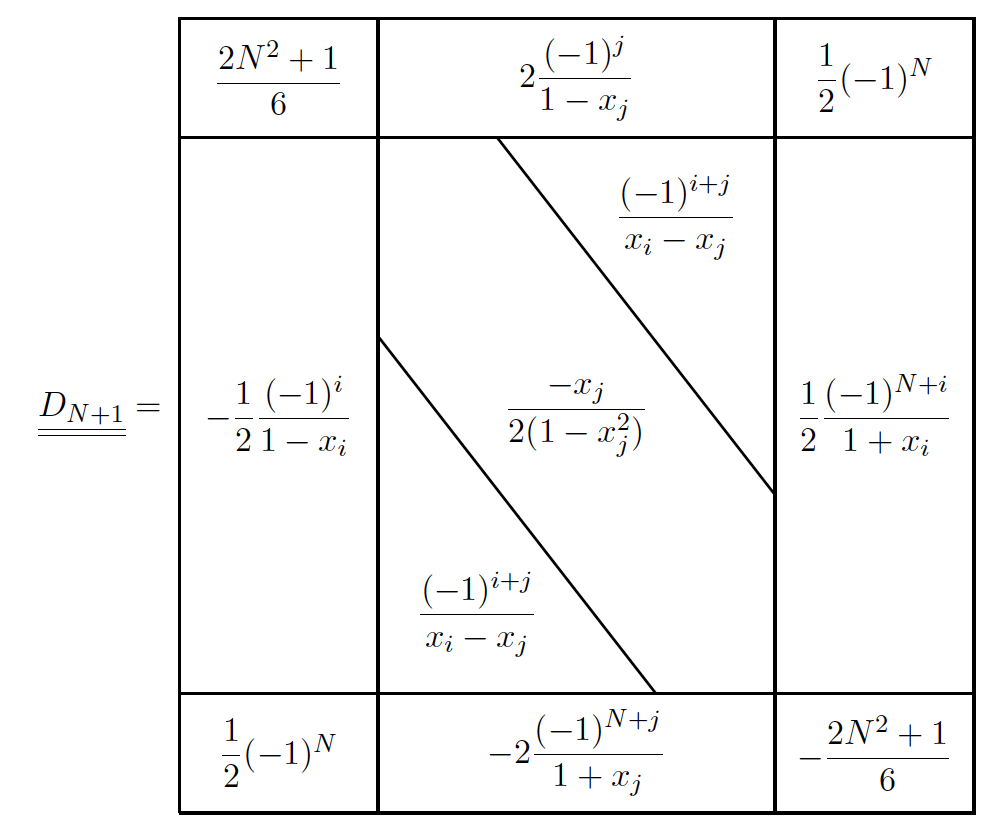
\includegraphics[scale=0.5]{figures/Chebyshev.jpg}
% 	\caption{This differentitation matrix works with chebyshev points.\cite{Peterson:2}\cite{Trefethen:7}}
% \end{figure}
\par
Thus, 
\begin{align}
    \vec{W_{p}}_{, t} + \lambda_{p} \, \vec{W_{p}}_{, s} = \sum_{q=1}^{M} F_{pq} \, \vec{W_{q}} \quad \rightarrow \quad
    \vec{W_{p}}_{, t} + \lambda_{p} \, \mat{D} \, \vec{W_{p}} = \sum_{q=1}^{M} F_{pq} \, \vec{W_{q}}
\end{align}
As usual, we need to also enforce boundary conditions (in particular, Dirichlet boundary conditions).
Since we are working a system of hyperbolic PDEs, we enforce inflow conditions:
\begin{itemize}
    \item If $\lambda_{p} > 0$, we enforce left inflow boundary conditions
    \item If $\lambda_{p} < 0$, we enforce right inflow boundary conditions
\end{itemize}
We can enforce the above inflow boundary conditions by modifying the appropriate columns and rows of $\mat{D}$ in the $p^{th}$ equation:
\begin{itemize}
    \item If $\lambda_{p} > 0$, we zero out the last column and last row of $\mat{D}$
    \item If $\lambda_{p} < 0$, we zero out the first column and first row of $\mat{D}$
\end{itemize}
\textbf{Note:} The above enforcement scheme makes sense in this context because the Chebyshev points of the second kind are ordered in \textit{decreasing} order from $1$ to $-1$.
\par 
Thus,
\begin{align}
    \vec{W_{p}}_{, t} + \lambda_{p} \, \mat{D} \, \vec{W_{p}} = \sum_{q=1}^{M} F_{pq} \, \vec{W_{q}} \quad \rightarrow \quad
    \vec{W_{p}}_{, t} + \lambda_{p} \, \mat{D_{p}} \, \vec{W_{p}} = \sum_{q=1}^{M} F_{pq} \, \vec{W_{q}}
\end{align}

\subsubsection{Temporal Discretization of the PDE}

Recall that we spatially discretized the $p^{th}$ equation in the above system to obtain
\begin{align}
    \vec{W_{p}}_{, t} + \lambda_{p} \, \mat{D_{p}} \, \vec{W_{p}} = \sum_{q=1}^{M} F_{pq} \, \vec{W_{q}}
\end{align}
We have not yet temporally discretized the system, but we have more freedom with picking time-stepping methods.
For this project, we adapted a \textbf{third-order}, \textbf{L-stable} IMEX Runge-Kutta scheme presented in \cite{PieracciniPuppo:3}.
The scheme is given as follows:
\begin{itemize}
    \item We have knowledge of the solution vectors $\vec{W_{p}}^{(n)}$ at some initial time-step $n$ for each equation $p = 1, 2, \hdots, M$
    \item In the first stage, we perform the following updates for equations $p = 1, 2, \hdots, M$:
    \begin{align}
        \vec{W_{p}}^{(1)} & = \vec{W_{p}}^{(n)} - \Delta t \, a_{11} \, \lambda_{p} \, \mat{D_{p}} \, \vec{W_{p}}^{(1)} \label{time_stepping:line_1}
    \end{align}
    \item For each stage $i = 2, \hdots, \nu$ (where $\nu = 4$ is the last stage), we perform the following updates for equations $p = 1, 2, \hdots, M$:
    \begin{align}
        \vec{W_{p}}^{(i)} & = \vec{W_{p}}^{(n)} + \Delta t \, \sum_{l=1}^{i-1} \widetilde{a}_{il} \sum_{q=1}^{M} F_{pq} \vec{W_{q}}^{(l)} - \Delta t \, \sum_{l=1}^{i} a_{il} \, \lambda_{p} \, \mat{D_{p}} \, \vec{W_{p}}^{(l)} \label{time_stepping:line_2}
    \end{align}
    \item To obtain the solution vectors $\vec{W_{p}}^{(n+1)}$ at the next time-step $(n+1)$, we perform the following updates for equations $p = 1, 2, \hdots, M$:
    \begin{align}
        \vec{W_{p}}^{(n+1)} & = \vec{W_{p}}^{(n)} + \Delta t \, \sum_{i=1}^{\nu} \widetilde{w}_{i} \sum_{q=1}^{M} F_{pq} \, \vec{W_{q}}^{(i)} - \Delta t \, \sum_{i=1}^{\nu} w_{i} \lambda_{p} \mat{D_{p}} \, \vec{W_{p}}^{(i)} \label{time_stepping:line_3}
    \end{align}
\end{itemize}
% \begin{align}
%   \vec{W_{p}}^{(1)} & = \vec{W_{p}}^{(n)} - \Delta t \, a_{11} \, \lambda_{p} \, \mat{D_{p}} \, \vec{W_{p}}^{(1)} \label{time_stepping:line_1} \\
%   \vec{W_{p}}^{(i)} & = \vec{W_{p}}^{(n)} + \Delta t \, \sum_{l=1}^{i-1} \widetilde{a}_{il} \sum_{q=1}^{M} F_{pq} \vec{W_{q}}^{(l)} - \Delta t \, \sum_{l=1}^{i} a_{il} \, \lambda_{p} \, \mat{D_{p}} \, \vec{W_{p}}^{(l)} \label{time_stepping:line_2} \\
%     \vec{W_{p}}^{(n+1)} & = \vec{W_{p}}^{(n)} + \Delta t \, \sum_{i=1}^{\nu} \widetilde{w}_{i} \sum_{q=1}^{M} F_{pq} \, \vec{W_{q}}^{(i)} - \Delta t \, \sum_{i=1}^{\nu} w_{i} \lambda_{p} \mat{D_{p}} \, \vec{W_{p}}^{(i)} \label{time_stepping:line_3}
% \end{align}
% In \ref{time_stepping:line_1}, we perform this update for $p = 1, 2, \hdots, M$.
% In \ref{time_stepping:line_2}, we perform this update first for every $i = 2, \hdots, \nu$ then for every $p = 1, 2, \hdots, M$, where $\nu = 4$ is the last stage number.
% In \ref{time_stepping:line_3}, we perform this update for $p = 1, 2, \hdots, M$.

\subsubsection{Solving the System via the Matrix Exponential}

We can also solve the above system using the matrix exponential.
Recall that the $p^{th}$ equation in the spatially discretized system is given by
\begin{align}
    \vec{W_{p}}_{, t} + \lambda_{p} \, \mat{D_{p}} \, \vec{W_{p}} = \sum_{q=1}^{M} F_{pq} \, \vec{W_{q}}
\end{align}
We can rearrange the above to obtain
\begin{align}
    \vec{W_{p}}_{, t} = -\lambda_{p} \, \mat{D_{p}} \, \vec{W_{p}} + \sum_{q=1}^{M} F_{pq} \, \vec{W_{q}}
\end{align}
We can then compute the solution of the entire system at the final time $t_{f}$ via the matrix exponential:
\begin{align*}
    \begin{bmatrix}
        \vec{W_{1}} \\
        \vec{W_{2}} \\
        \vdots \\
        \vec{W_{M}}
    \end{bmatrix}
    & = \exp \left(-t_{f}
    \begin{bmatrix}
    -\lambda_{1} \, \mat{D_{1}} + F_{11} \, \mat{I} & F_{12} \, \mat{I} & \hdots & F_{1m} \, \mat{I}  \\
    F_{21} \, \mat{I} & -\lambda_{2} \, \mat{D_{2}} + F_{22} \, \mat{I} & \hdots & F_{2m} \, \mat{I}  \\
    \vdots & \vdots & \ddots & \vdots \\
    F_{m1} \, \mat{I} & \hdots & F_{m(m-1)} \, \mat{I} & -\lambda_{m} \, \mat{D_{m}} + F_{mm} \, \mat{I}
    \end{bmatrix} \right)
    \vec{W_0}
\end{align*}
where
\begin{align}
    \vec{W_{0}} & =
    \begin{bmatrix}
        \vec{W_{1}}^{(0)} \\
        \vec{W_{2}}^{(0)} \\
        \vdots \\
        \vec{W_{m}}^{(0)}
    \end{bmatrix} \in \mathbb{R}^{(M \cdot N_{s})}
\end{align}
is a vector of discretized initial conditions corresponding to the $M$ equations in the system.  